\section{Scopi e servizi}
I protocolli a livello di trasporto mettono a disposizione una \textbf{comunicazione logica} tra processi applicativi di due host diversi. Sono 
implementati nei sistemi periferici; lato client, il livello di trasporto converte i messaggi spezzettandoli in \textbf{segmenti} e aggiungendo loro 
un'\textbf{intestazione}; il prodotto è passato al livello di rete che li incapsulerà in un pacchetto detto \textbf{datagramma} e inviato a destinazione.\par
Lato server, invece, il livello di rete estrae i segmenti dai datagrammi ottenuti e li passa al livello di trasporto, il quale li elabora, estraendo 
i dati per renderli disponibili all'applicazione destinataria.\newline

\noindent Come già menzionato in precedenza, il livello di trasporto fornisce due protocolli: \begin{itemize}
	\item \textbf{Transmission Control Protocol} (TCP): Servizio orientato alla connessione, che garantisce la consegna ordinata di tutti i segmenti.
	\item \textbf{User Datagram Protocol} (UDP): Servizio non orientato alla connessione, non affidabile.
\end{itemize}
\noindent Entrambi separano il messaggio originale in segmenti e aggiungono un'intestazione di forma diversa, la quale sarà trattata nelle seguenti
sezioni. Prima di discuterne è tuttavia necessario chiarire in che modo i dati vengono trasferiti, ovvero come il servizio di trasporto a livello di
rete possa diventarne un'altro da processo a processo per le applicazioni.\par
Ricordiamo che il livello di trasporto invia i dati agli host tramite un socket, il quale ha un identificatore univoco il cui formato dipende dal
protocollo utilizzato. Ciascun segmento dei dati originali presenta vari campi; lato ricevente, il livello di trasporto li analizza per identificare
il socket di ricezione e dirigervi il segmento. Definiamo questo compito \textbf{demultiplexing}, mentre il suo duale, ovvero il raggruppare i segmenti
ed incapsularli con un'intestazione per inviarli al livello di rete, è detto \textbf{multiplexing}. Con questi presupposti possiamo ora analizzare nel
dettaglio i due protocolli di trasporto.

%

\section{Protocollo TCP}
Il \textbf{Transport Control Protocol} (TCP) è un protocollo orientato alla connessione perché richiede un preliminare scambio di messaggi per la sua
instaurazione, ed è ritenuto affidabile in quanto si assicura la consegna ordinata di ogni dato tramite ricevute inviate dall'end-host ricevente.\par
Supponiamo ora che il processo di un host voglia comunicare con un altro; in primo luogo, l'applicativo del client informerà il suo livello di trasporto
di voler stabilire una connessione verso un processo nel server e gli invierà quindi un segmento TCP. Il server risponderà con un altro segmento, alla
cui ricezione da parte del client, ne invierà un terzo. Inviando tre segmenti, questa fase è detta \textbf{three-way handshake} e le sue specifiche
saranno trattate nel dettaglio più avanti nella sezione.\par
Instaurata una connessione TCP, i due processi applicativi potranno scambiarsi i dati bidirezionalmente tramite il socket aperto, in base ad un valore
specifico, detto \textbf{maximum segment size} (MSS), che indica la massima quantità di dati prelevabili e posizionabili in un singolo segmento a
livello di applicazione. È un valore impostato nel three-way handshake determinando la lunghezza del frame più grande che può essere inviato a livello
di collegamento, la \textbf{maximum transmission unit} (MTU).\par
TCP accoppierà poi ogni blocco di dati (\textbf{payload}) ricevuto dal livello superiore con un'\textbf{intestazione TCP}, formando i segmenti da
inviare a livello di rete, ivi incapsulati a loro volta in \textbf{datagrammi IP}. Quando l'end-host ricevente riceve un segmento, i suoi dati sono
memorizzati in un buffer di ricezione il quale è letto dal livello applicativo.\newline

\noindent Analizziamo nel dettaglio la struttura dell'intestazione TCP; comunemente occupa $20B$ e presenta i seguenti campi: \begin{itemize}
	\item \textbf{Porta sorgente/destinazione}: Identificatori dei processi coinvolti nella comunicazione. Ciascuno di questi valori è rappresentato
	da $16b$, rendendo possibile usare $65536$ porte diverse, le quali si dividono in due tipi: \begin{itemize}
		\item \textbf{Statiche}: Identificativi utilizzabili esclusivamente lato server associati a protocolli definiti da uno standard come HTTP o
		SMTP. Comprendono i valori dell'intervallo $[0, 1023]$.
		\item \textbf{Dinamiche}: Identificativi assegnati dal sistema operativo al lato client quando viene aperto un socket. Prendono un numero
		casuale dall'intervallo $[1024, 65535]$.
	\end{itemize}
	\item \textbf{Numero di sequenza/acknowledgement}: Utilizzati per implementare l'affidabilità del protocollo, richiedono entrambi $32b$. Il numero
	di sequenza indica l'offset rispetto al primo byte del segmento e consente di capire come devono essere ricostruiti\footnote{Supponiamo di avere un
	messaggio di dimensione $5000B$ e che l'MSS sia di $900B$. Il primo segmento avrà $0$ come numero di sequenza, il secondo $900$, il terzo $1800$ e
	così via.}. L'offset è calcolato sommando un \textbf{initial sequence number}, un numero casuale generato dal sistema operativo che rimane
	costante, con il numero di sequenza del segmento. Il numero di acknowledgement indica invece il primo byte del segmento che la destinazione si
	aspetta di ricevere.
	\item \textbf{Offset intestazione}: Specifica la lunghezza dell'intestazione TCP in multipli di $32b$.
	\item \textbf{Flag}: Questo campo contiene dei segnalatori con logica di codifica 1-hot. \textbf{ACK} segnala che un segmento contiene un
	acknowledgement per un segmento ricevuto correttamente. \textbf{RST}, \textbf{SYN} e \textbf{FIN} sono invece usati per impostare e chiudere la
	connessione. L'insieme richiede $6b$.
	\item \textbf{Finestra di ricezione}: Usata per il controllo di flusso, indica il numero di byte che il destinatario è disposto ad accettare.
	Richiede $16b$.
	\item \textbf{Checksum Internet}: Richiesto per il controllo di errori nel segmento. Si chiama una funzione che prende l'intestazione come input;
	il suo output è assegnato a questo campo. Si tratta di un controllo attuabile da entrambi gli host e se l'output risultante è lo stesso, è altamente
	probabile che i dati siano corretti. Se differiscono, il segmento è scartato.
	\item \textbf{Opzioni}: Facoltativo e di lunghezza variabile, è utilizzato quando i due host devono determinare la lunghezza dell'MSS.
\end{itemize}
\noindent Definita l'intestazione, ora possiamo andare più nel dettaglio in merito all'instaurazione delle connessioni TCP. Il three-way handshake si
compone di più elementi: in primo luogo, di un messaggio di \textbf{sincronizzazione} inviato dal client, contenente i parametri delle porte, numero di
sequenza, numero di acknowledge e il flag SYN posto a $1$. Segnala la volontà di aprire una connessione.\par
Il server risponderà con un messaggio di acknowledge sincronizzazione, dove sono contenuti i parametri delle porte invertiti, l'ISN$_s$\footnote{
	Indichiamo $ISN_c$ e $ISN_s$ come initial sequence numbers di client e server rispettivamente. In particolare, $ISN_s=ISN_c+1$.
	}, acknowledge number e naturalmente i flag SYN e ACK posti a $1$.\par
La stretta di mano si conclude con un messaggio di acknowledge da parte del client, il quale invierà i parametri delle porte, l'ISN$_c$, il flag ACK
posto a $1$ e come numero di acknowledge il valore $ISN_s+1$.\newline
\begin{figure}[h]
	\centering
	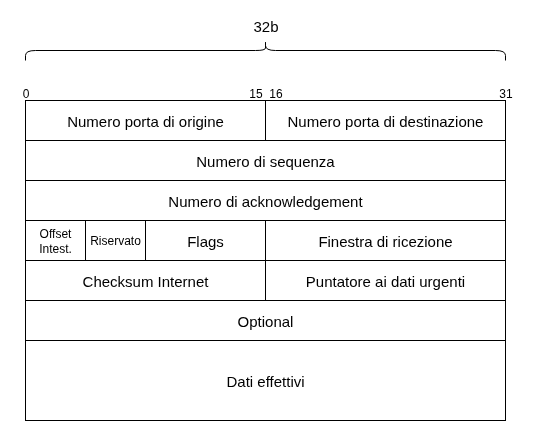
\includegraphics[width=0.75\linewidth]{Images/headerTCP.png}
	\caption{Intestazione dei segmenti TCP}
\end{figure}

\noindent Durante il three-way handshake è inoltre deciso il parametro di maximum segment size per evitare che si sforino le capacità delle schede di
rete, ed è scelto il valore più piccolo delle due entità.\par
La richiesta di chiusura della connessione, come per il suo duale, richiede uno scambio di messaggi di header TCP, ed è una procedura che avviene
indipendentemente nei due host. Si utilizzano messaggi di FIN e ACK con i relativi flag posti a $1$ e possono avvenire i seguenti casi: \begin{itemize}
	\item Se il client è il primo a inviare un FIN, il server ritornerà un ACK e la connessione sarà chiusa lato client. L'altro host invierà poi a sua
	volta il FIN ed il client risponderà con un ACK. La connessione si può considerare chiusa solo dopo questo scambio.
	\item Il primo host invia un messaggio di FIN e il secondo ritornerà un ACK, chiudendo una direzione del socket. Quando la procedura è ripetuta in
	viceversa, la connessione TCP sarà del tutto chiusa.
	\item Una procedura più rapida vede il primo host inviare un FIN ed il secondo ritornare un FIN-ACK. Ricevuto quest'ultimo messaggio, il primo host
	risponderà con un ACK a sua volta, chiudendo la connessione.
\end{itemize}

\noindent Chiediamoci adesso quali siano le modalità procedurali che rendono il TCP un protocollo affidabile. Adotta in primo luogo la tecnica del
\textbf{positive acknowledgement with retransmission}, dunque ad ogni segmento inviato deve corrispondere un responso positivo dall'altro host.
Quando non è ricevuto, si ritenta l'invio fino a quando non lo si ottiene.\par
Il riscontro è un messaggio di acknowledgement che, come detto prima, contiene il relativo flag posto ad $1$ ed il primo byte del segmento che la
destinazione si aspetta di ricevere. Ciò significa che se lato client è stato inviato un sequence number $44$, il numero di acknowledge inviato dal
server sarà $45$. Quando non è ricevuto questo valore, si attiva un timer chiamato \textbf{Retransmission Time-out} (RTO), al termine del quale si invia
nuovamente il messaggio precedentemente non corrisposto.\par
Il valore di RTO è inizialmente posto a $5000ms$ preventivando eventuali problemi legati a fattori come distanza geografica o problemi di rete. Non è
tuttavia un numero fisso; infatti, client e server misurano il Roundtrip time ad ogni segmento inviato e usano il primo come base di calcolo per 
aggiornare una variabile chiamata \textbf{smoothed-RTT} (SRTT) oppure Exponential Weighted Moving Average (EWMA) secondo la formula: \[
SRTT_{\text{attuale}} = \alpha SRTT_{\text{precedente}} + (1-\alpha)RTT_{\text{istantaneo}} \quad\text{con $0 < \alpha < 1$}
\]
\noindent SRTT è una stima del valore medio di Roundtrip time e si utilizza per calcolare l'RTO con la formula: \[
RTO = \beta\cdot SRTT\quad\text{con $\beta$ generalmente uguale a $2$}
\]
\noindent Il quale, in caso di perdita di un segmento, è raddoppiato. Questo meccanismo è necessario perché potremmo trovarci nelle condizioni di
inviare segmenti ad un'applicazione con bassa velocità di lettura del suo buffer di ricezione, ma allora dovremmo rallentare la velocità di trasmissione,
facendo risultare la connessione più lenta. Come è possibile avere un'alta velocità di trasmissione senza mandare il buffer in overflow?\par
Le risposte offerte dal protocollo TCP vengono nella forma di \textbf{controllo di flusso} e \textbf{controllo di congestione}; il primo è un'azione
preventiva per evitare la congestione e riduce la probabilità di perdere dei segmenti, mentre il secondo è una reazione in caso di congestione della
rete, dunque quando non si ricevono riscontri per i segmenti inviati.\newline

\noindent Il controllo di flusso è un meccanismo che consente anche l'invio di più segmenti alla volta grazie all'implementazione di una \textbf{
finestra di ricezione scorrevole} (RCVWND) con un relativo parametro che salva la sua dimensione. Si tratta del numero massimo di segmenti inviabili
al buffer del destinatario; se per esempio la dimensione corrisponde a tre segmenti, il mittente potrà inviare i segmenti $s1, s2, s3$ in una volta
sola, alla cui ricezione da parte del server, risponderà con tre numeri di acknowledge di fila. Ad ogni riscontro ricevuto, la finestra si sposterà
di una posizione, per consentire l'invio dei segmenti successivi, fino alla consegna dell'intero pacchetto. La formula della velocità di trasmissione
diventa quindi: \[
v_t = RCVWND / RTT
\]

\begin{figure}[h]
	\centering
	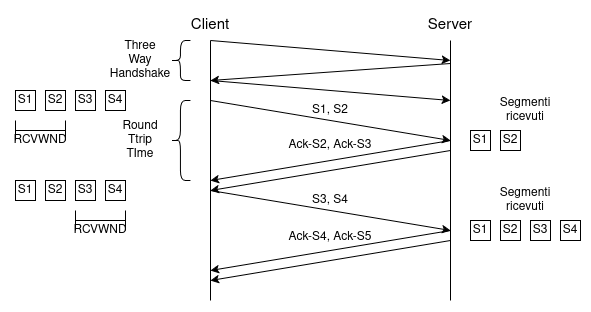
\includegraphics[width=0.75\linewidth]{Images/streamControl.png}
	\caption{Esempio controllo di flusso}
\end{figure}

\noindent Non sempre si può ottenere il caso ideale appena discusso; è possibile avere \textbf{perdite} o \textbf{ritardi} di segmenti durante i
tentativi della loro trasmissione. Per il primo scenario supponiamo che il client voglia inviare una sequenza di tre segmenti $s1, s2, s3$ e che il
terzo venga perso per qualche motivo.\par
In tal caso, il server ritornerà correttamente i numeri di acknowledge per i primi due segmenti senza inviare l'ultimo. L'RTO per il terzo segmento
è quindi ancora attivo. Ricevuti i riscontri, la finestra di ricezione si sposterà di due posizioni e il client potrà inviare i successivi due elementi
$s4, s5$, correttamente ricevuti dal server, il quale continuerà a ritornare l'acknowledge number per il segmento mancante: $ack3$. Il mittente
attenderà quindi lo scadere dell'RTO per ritrasmettere il segmento $s3$, ed una volta recepito dal server, ritornerà $ack6$, poiché ha già ricevuto
tutti i segmenti fino a $s5$.\par
Generalmente, quando un server riceve pacchetti diversi da quelli comunicati tramite l'acknowledge number, continua a reinviare quest'ultimo fino a
quando non è recepito. In caso di ritardi infatti, se un client invia tre segmenti $s1, s2, s3$ come prima, ma il secondo ha un ritardo, il server
invierà $ack2$ fino a quando non gli sarà consegnato.\newline

\begin{figure}[h]
	\centering
	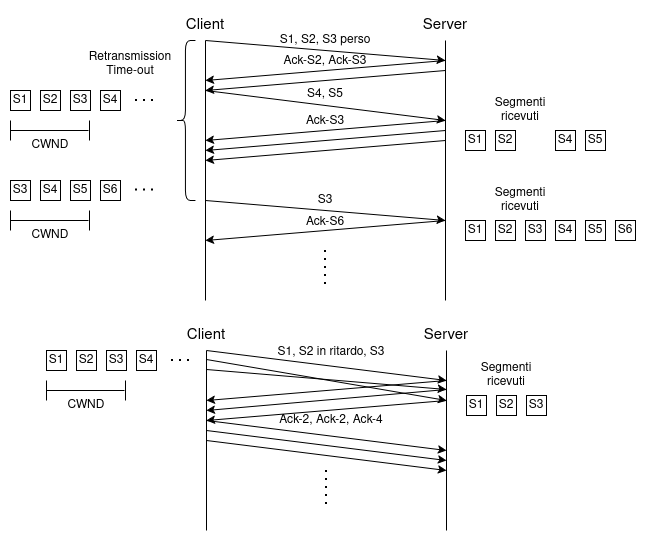
\includegraphics[width=0.75\linewidth]{Images/streamControlProblems.png}
	\caption{Perdita e ritardo di pacchetti}
\end{figure}

\noindent Ma in che modo è determinata la dimensione della finestra di trasmissione? Non è possibile avere un valore determinato, bisogna infatti
adattarlo in base alla situazione corrente della rete. Ciò avviene grazie ai riscontri; la loro ricezione o assenza è il metro per l'adattamento.\par
In genere, se i riscontri sono ricevuti regolarmente, è un segnale che la rete è in grado di gestire il traffico inviato e si potrebbe pensare di
aumentare la dimensione della finestra. In caso contrario, quindi in presenza di perdite, alla scadenza dell'RTO ne si diminuisce la dimensione.
Le regole per la gestione di questo meccanismo sono: \begin{itemize}
	\item \textbf{Slow-Start}: Oltre a spostare la finestra, aumenta la sua dimensione di un segmento per ogni riscontro correttamente ricevuto.
	\item \textbf{Congestion avoidance}: Ad ogni riscontro ricevuto, aumenta la dimensione della finestra di $1/w$. Per esempio, partendo con una
	dimensione $w=2$, alla ricezione dei due riscontri si incrementa la grandezza di $2\cdot 1/2 = 1$ segmento. 
	\item \textbf{Vanilla TCP}: Quando non si è ricevuto un riscontro entro l'RTO, la dimensione è ridotta a $1$ e si ricomincia la trasmissione a
	partire dal segmento perso.
	\item \textbf{Fast retransmit/Fast recovery}: Quando non si è ricevuto un riscontro entro l'RTO, si dimezza\footnote{Generalmente si approssima
	il risultato per difetto, ma è contemplata, previa segnalazione, l'approssimazione per eccesso.} la dimensione attuale della finestra
	e si ricomincia la trasmissione a partire dal segmento perso.
\end{itemize}

\noindent Viene usato un \textbf{algoritmo} specifico per il \textbf{controllo} della \textbf{congestione} e richiede i parametri discussi prima:
congestion window (CWND), la dimensione della finestra; retransmissione time-out (RTO); receiver window (RCVWND), la finestra massima di ricezione
segmenti; slow-start threshold (SSTHRESH), soglia per determinare l'utilizzo di slow-start o congestion avoidance.
\begin{algorithm}
	\caption{TCP-WindowManager()}
	\begin{algorithmic}[i]
		\State $cwnd\gets 1$
		\State $rcvwnd\gets$ valore comunicato ad ogni riscontro
		\State $ssthresh\gets rcvwnd$
		\State $rto\gets$ valore misurato con $\beta\cdot SRTT$
		\State
		\State Client invia un numero $cwnd$ di segmenti
		\If{Riscontro ricevuto}
		\If{$cwnd < ssthresh$} \Comment{Uso lo slow-start}
		\State $cwnd\gets min(cwnd + ackNum, rcvwnd, ssthresh)$
		\Else \Comment{Uso la congestion avoidance}
		\State $cwnd\gets min(cwnd+ackNum / cwnd, rcvwnd)$
		\EndIf
		\Else \Comment{Se non arrivano riscontri e scade l'RTO}
		\State $ssthresh\gets cwnd/2$
		\State $cwnd\gets 1$ \Comment{In caso di vanilla TCP}
		\State $rto\gets 2*rto$
		\EndIf
	\end{algorithmic}
\end{algorithm}

\begin{figure}[h]
	\centering
	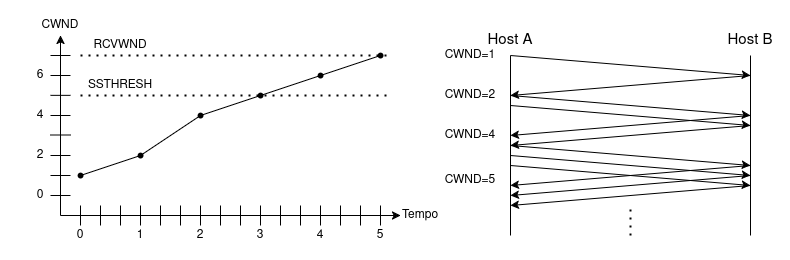
\includegraphics[width=0.9\linewidth]{Images/congestionControl.png}
	\caption{Panoramica algoritmo controllo congestione}
\end{figure}

%

\section{Protocollo UDP}
Il protocollo \textbf{User Datagram Protocol} (UDP) ha una struttura nettamente più semplice rispetto al TCP: diciamo anzitutto che è \textbf{
connectionless} perché non effettua un preliminare scambio dei messaggi prima di inviare dati al server. UDP riceve i messaggi, aggiunge porta di
origine e destinazione e passa il segmento a livello di rete, dove viene incapsulato e inviato in modalità "best-effort". Ciò significa che non è
garantita la consegna dei segmenti, rendendolo un protocollo inaffidabile.\par
Tuttavia, non significa che non abbia comunque i suoi utilizzi. UDP è un protocollo utilizzato per le applicazioni \textbf{tolleranti alle perdite}
grazie ad alcuni suoi pregi: \begin{itemize}
	\item Richiede un controllo più preciso a livello applicativo su quali dati sono inviati e quando.
	\item In quanto connectionless, non genera un ritardo per l'instaurazione della connessione.
	\item Richiede minor spazio per l'intestazione dei pacchetti.
\end{itemize}

\noindent Quindi, sebbene a primo impatto possa sembrare inutilizzabile, UDP è un protocollo importante per il funzionamento di molte applicazioni
che richiedono tempi di risposta rapidi e in tempo reale. Per esempio, in quelle di streaming audio si riceve il segnale, che è quantizzato e
discretizzato, per poi essere diviso in pacchetti ai quali è aggiunto l'header. Vengono inviate al secondo host, il quale potrà ricostruirlo
ordinatamente, ma in caso di perdita, lascerà del silenzio. La velocità di trasmissione dei dati dipende quindi dalla loro velocità di generazione.\par
L'header, come già detto, di dimensione minore rispetto al TCP, presenta quattro campi: porta di origine, porta di destinazione e checksum, il cui
funzionamento è identico al TCP, e quello di \textbf{lunghezza dei dati} per indicare la loro dimensione.

\begin{figure}[h]
	\centering
	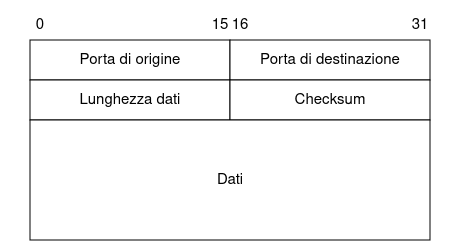
\includegraphics[width=0.6\linewidth]{Images/UDP_header.png}
	\caption{Panoramica intestazione UDP}
\end{figure}

%

\section{Esercizi svolti}
\textbf{Esercizio 1}: Sia un'applicazione A che desidera trasferire $96000B$ ad una seconda applicazione B. Si suppone che la connessione sia già
instaurata e presenti i seguenti parametri: \begin{itemize}
	\item Maximum Segment Size: $1000B$.
	\item Receive Window: $32000B$, rimane costante per tutta la trasmissione.
	\item Slow Start Threshold: $\text{RCVWND}_i/2$.
	\item Round-trip time: $0,5s$, rimane costante per tutta la trasmissione.
	\item Retransmission time-out: $2RTT$, raddoppia in caso di perdite sequenziali.
\end{itemize}
\noindent Sono inoltre presenti dei down di rete durante gli intervalli di tempo $(3, 3.5), (7, 7.5)$. Valutare l'evoluzione temporale della congestion
window fino al termine della trasmissione.\par
Lo svolgimento di questo esercizio è dato interamente dall'algoritmo di slow start, per il quale valgono le seguenti regole generali: \begin{itemize}
	\item La dimensione della congestion window aumenta esponenzialmente finché il valore è minore dello slow start threshold.
	\item Arrivati ad un valore maggiore o uguale al threshold, si pone il valore di quest'ultimo alla finestra, per poi procedere aumentando la sua
	dimensione di 1 ad ogni RTT.
	\item Con eventuali down di rete, il threshold ottiene il valore dato dal rapporto tra dimensione della finestra corrente e 2, poi la dimensione
	della finestra torna a 1. Inoltre, si potrà ricominciare a trasmettere solo dopo un RTO.
\end{itemize}
\noindent Sapendo questo, iniziamo ottenendo il valore in segmenti dei dati da trasmettere, dividendo i Byte totali con la MSS: \[
	\text{Segmenti: } 92000/1000 = 92,\quad \text{RCVWND: } 32000/1000=32,\quad \text{SSTHR: } 32/2 = 16
\]
\noindent Se disegnato correttamente, l'evoluzione temporale è la seguente: \begin{itemize}
	\item $1+2+4+8+16+17+18(0) = 48$. I 18 segmenti sono trasmessi ma non sono stati recepiti a causa del down di rete. Non è stato quindi ricevuto
	alcun acknoledgement. Si attiva l'RTO, si pone $\text{SSTHR}_2=18/2=9$ e $CWND=1$.
	\item $48+1+2+4+8+9+10+11(0) = 82$. Gli 11 segmenti hanno subito la stessa sorte sovramenzionata causa down di rete. Scaduto l'RTO, abbiamo che
	$\text{SSTHR}_3=11/2=4,5$ e $CWND=1$. L'approssimazione del treshold è arbitraria, previa segnalazione si può approssimare per eccesso o difetto. In
	questo esempio, approssimiamo per difetto, quindi $\text{SSTHR}_3=4$.
	\item $82+1+2+4+5+(6-4) = 96$. La dimensione finale della congestion window risulta come: \[
		\text{CWND}_f = \text{CWND}_c + \text{ackRicevuti}/\text{CWND}_c = 6 + 2/6 = 6,33 = 6
	\]
	\noindent L'ultimo acknowledge è poi ricevuto con il termine del round-trip time attivato con l'invio degli ultimi $(6-4)=2$ segmenti. Il tempo di
	trasmissione totale è quindi $t=10,5s$
\end{itemize}
\begin{figure}[h]
	\centering
	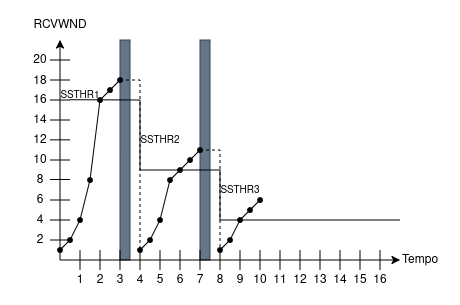
\includegraphics[width=0.75\linewidth]{Images/tcp_ex1.png}
	\caption{Evoluzione trasmissione esercizio 1}
\end{figure}

\noindent \textbf{Esercizio 2}: Sia un'applicazione A che desidera trasferire $46500B$ ad una seconda applicazione B. Si suppone che la connessione sia
già instaurata e presenti i seguenti parametri: \begin{itemize}
	\item Maximum Segment Size: $1500B$.
	\item Receive Window: $24000B$, rimane costante per tutta la trasmissione.
	\item Slow Start Threshold: $\text{RCVWND}_i/2$.
	\item Round-trip time: $0,5s$, rimane costante per tutta la trasmissione.
	\item Retransmission time-out: $2RTT$, raddoppia in caso di perdite sequenziali.
\end{itemize}
\noindent Sono inoltre presenti dei down di rete durante gli intervalli di tempo $(1.5, 3.5), (7, 7.5)$. Valutare l'evoluzione temporale della
congestion window fino al termine della trasmissione.\par
Stesso identico procedimento di prima; trasformiamo i Byte in segmenti: \[
	\text{Segmenti: } 46500/1500 = 31,\quad \text{RCVWND: } 24000/1500=16,\quad \text{SSTHR: } 16/2 = 8
\]
\noindent Se disegnato correttamente, l'evoluzione temporale è la seguente: \begin{itemize}
	\item $1+2+4+8(0)=7$. Gli 8 segmenti sono stati persi a causa del down di rete. poniamo $\text{SSTHR}_2=8/2=4$ e $CWND=1$; parte inoltre l'RTO, ma
	non è sufficiente per superare il problema. Si raddoppia, quindi, arrivando a $RTO=2s$, dimezzando ulteriormente il threshold. Si supera il down.
	\item $7+1+2+3+4+5+6(0)=22$. I 6 segmenti subiscono la medesima sorte. $\text{SSTHR}_4=6/2=3$, $CWND=1$. Riparte di nuovo l'RTO di $1s$.
	\item $22+1+2+3+(4-1) = 31$. All'ultima finestra rimanevano solo 3 segmenti da trasmettere.
\end{itemize}
\noindent Dimensione finale della CWND$_f=4+3/4=4,75$, tempo di trasmissione totale $t=10s$ al termine della ricezione dell'ultimo acknowledgement.
\begin{figure}[h]
	\centering
	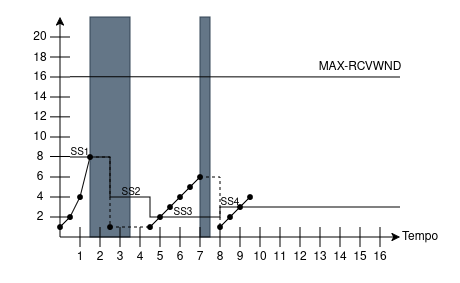
\includegraphics[width=0.75\linewidth]{Images/tcp_ex2.png}
	\caption{Evoluzione trasmissione esercizio 2}
\end{figure}

\noindent \textbf{Esercizio 3}: Sia un'applicazione A che desidera trasferire $104000B$ ad una seconda applicazione B. Si suppone che la connessione sia
già instaurata e presenti i seguenti parametri: \begin{itemize}
	\item Maximum Segment Size: $1200B$.
	\item Receive Window: $24000B$, rimane costante per tutta la trasmissione.
	\item Slow Start Threshold: $\text{RCVWND}_i$.
	\item Round-trip time: $0,5s$, rimane costante per tutta la trasmissione.
	\item Retransmission time-out: $2RTT$, raddoppia in caso di perdite sequenziali.
\end{itemize}
\noindent Sono inoltre presenti dei down di rete durante gli intervalli di tempo $(3.5, 4), (6.5, 10.5)$. Valutare l'evoluzione temporale della
congestion window fino al termine della trasmissione. Non credo ci sia bisogno di ripetermi, no? \[
	\text{Segmenti: } 104000/1200 = 87,\quad \text{RCVWND: } 24000/1200=20 = \text{SSTHR}
\]
\noindent Trasmissione: \begin{itemize}
	\item $1+2+4+8+16+20+20+20(0) = 71$. Down di rete. You know the drill.
	\item $71+1+2+4+8+10(0) = 86$. Grosso down di rete ora. Tre volte scade l'RTO, diventando uguale a $4s$ e la SSTHR è ridotta a $2$ segmenti.
	\item $86+1 = 87$.
\end{itemize}
\noindent Dimensione finale della CWND: $2 + 1/2=2.5$, tempo di trasmissione totale: $t=14s$.
\begin{figure}[h]
	\centering
	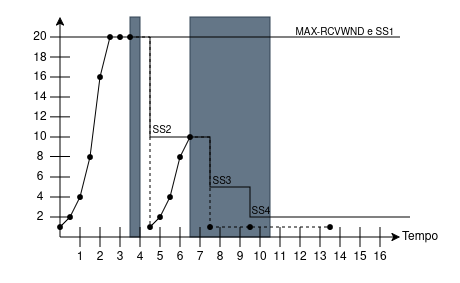
\includegraphics[width=0.6\linewidth]{Images/tcp_ex3.png}
	\caption{Evoluzione trasmissione esercizio 3}
\end{figure}

\begin{comment}
--- TCP esercizio 4
AppA deve trasferire 104400B verso AppB
MSS = 1200B
RCVWND_i = 9600B
A partire dall'istante t_a > 4s, la destinazione annuncia una RCVWND = 14400B
A partire dall'istante t_b > 9s, la destinazione annuncia una RCVWND = 7200B
SSTHRESH_i = RCVWND_i // Occhio quindi non è influenzata dalle successive ridefinizioni della RCVWND
CWND = 1	
RTT = 1s costante per tutta la trasmissione
RTO = 2RTT
Down di rete in intervallo (11.5, 12.5)

// Tip: le modifiche alla RCVWND sono comunicate dalla destinazione e il grafico che facciamo riguarda la sorgente. Quindi non le si riceve esattamente
agli istanti t_a, t_b, bensì alla ricezione dell'ack.
// Tip: A causa del down di rete, sono correttamente inviati i pacchetti, ma non si riceve il relativo ack. In quanto tale, si attiva ugualmente l'RTO.

--- Soluzione esercizio TCP 4
AppA deve trasferire 104400B verso AppB
MSS = 1200B
RCVWND_i = 9600B
A partire dall'istante t_a > 4s, la destinazione annuncia una RCVWND = 14400B
A partire dall'istante t_b > 9s, la destinazione annuncia una RCVWND = 7200B
SSTHRESH_i = RCVWND_i // Occhio quindi non è influenzata dalle successive ridefinizioni della RCVWND
CWND = 1
RTT = 1s costante per tutta la trasmissione
RTO = 2RTT
Down di rete in intervallo (11.5, 12.5)

// Tip: le modifiche alla RCVWND sono comunicate dalla destinazione e il grafico che facciamo riguarda la sorgente. Quindi non le si riceve esattamente agli istanti t_a, t_b, bensì alla ricezione dell'ack.
// Tip: A causa del down di rete, sono correttamente inviati i pacchetti, ma non si riceve il relativo ack. In quanto tale, si attiva ugualmente l'RTO.

RCVWND_1: 9600B/1200B = 8
RCVWND_2: 14400B/1200B = 12
RCVWND_3: 7200B/1200B = 6
Segmenti da trasmettere: 104400B/1200B = 87
Segmenti trasmessi: 1+2+4+8+8+9+10+11+12+12+6+0 = 83 // Down di rete, i 4 segmenti rimanenti non sono inviati.
Segmenti trasmessi: 1+2+(4-3) = 87

Tempo totale = 16s, CWND finale: 3+1/3.

In caso di perdita dei segmenti va così, mentre in caso di perdita dei riscontri durante il down di rete, non avendo ricevuto conferma, è necessario aspettare il termine dell'RTO per una ritrasmissione a t=13s.
Si cambia ovviamente la SSTHRESH e la CWND. Si ritrasmette il primo segmento, ma la destinazione aveva già ricevuto quelli trasmessi prima del down, quindi verrà ritornato un ack88. La sorgente si rende conto che i segmenti erano stati trasmessi correttamente, ricalcola il nuovo valore della CWND = CWND+ackReceived = 1+1 = 2 e chiuderà la connessione, facendo terminare la trasmissione a t=14s.


--- Esercizio TCP
AppA deve trasferire 77500B verso appB
MSS: 1250B
RCVWND a t=0: 10000B. A t>4 dst annuncia RCVWND di 17500B. A t>8 dst annuncia RCVWND di 12500B.
SSTHRESH_i: RCVWND_i
RTT = 1s costante per tutto il trasferimento e RTO = 2RTT e raddoppia in caso di perdite.
Rete down: (8, 10) e (13.5, 14.5)

RCVWND_1 = 8, RCVWND_2 = 14, RCVWND_3 = 10
SEGMENTI: 62

Inviati: 1+2+4+8+8+9+10+11+9(0) = 53 // 9 non inviato, down di rete.
Inviati: 53 + 1+2+4+6(0) = 60
Inviati: 60 + 1+1, fine trasmissione a t=17ms con CWND=3
\end{comment}